\documentclass{standalone}
\usepackage[utf8x]{inputenc}
\usepackage{tikz} 
\usepackage{varwidth}
\usepackage{ragged2e}
% \usepackage{pgfplots,pgfplotstable}
\usepackage{color}

\usetikzlibrary{arrows,positioning} 
\definecolor{myorange}{RGB}{230,97,1}
\definecolor{mylightorange}{RGB}{253,184,99}
\definecolor{mypurple}{RGB}{94,60,153}
\definecolor{mylightpurple}{RGB}{178,171,210}
\definecolor{mycolor1}{RGB}{35,139,69}
\definecolor{mycolor2}{RGB}{102,194,164}
\definecolor{mycolor3}{RGB}{178,226,226}
\definecolor{mycolor4}{RGB}{237,248,251}

\begin{document}

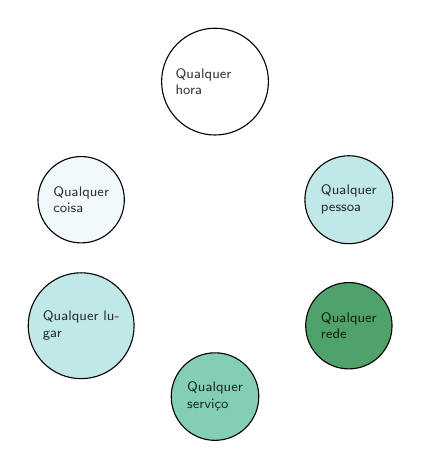
\begin{tikzpicture}[font=\sffamily]
      \begin{scope}[shift={(0cm,0cm)}, fill opacity=0.8]
        \node[draw,circle,scale=1, text width=1cm] 
        at (0,0) {\begin{varwidth}{1cm}\tiny{Qualquer hora}\end{varwidth}};
      
        \node[draw,circle,scale=1, fill=mycolor4] 
        at (-1.7,-1.5) {\begin{varwidth}{1cm}\tiny{Qualquer coisa}\end{varwidth}};

        \node[draw,circle,scale=1, fill=mycolor3] 
        at (-1.7,-3.1) {\begin{varwidth}{1cm}\tiny{Qualquer lugar}\end{varwidth}};

        \node[draw,circle,scale=1, fill=mycolor2] 
        at (0,-4) {\begin{varwidth}{1cm}\tiny{Qualquer serviço}\end{varwidth}};

        \node[draw,circle,scale=1, fill=mycolor1] 
        at (1.7,-3.1) {\begin{varwidth}{1cm}\tiny{Qualquer rede}\end{varwidth}};

        \node[draw,circle,scale=1, fill=mycolor3] 
        at (1.7,-1.5) {\begin{varwidth}{1cm}\tiny{Qualquer pessoa}\end{varwidth}};
      \end{scope}
\end{tikzpicture} 

\end{document}
